% Source: graduate-coursework/Sp26/CSCE763/Course_Assignments/Project/project_proposal.tex
% Description: Two-level 2D wavelet decomposition (DWT layout shown for clarity; SWT preserves full spatial resolution). Target energy concentrates in detail sub-bands ({\color{USC_Garnet

\documentclass[border=4pt]{standalone}
\usepackage{amsmath}
\usepackage{amssymb}
\usepackage{graphicx}
\usepackage{tikz}
\usepackage{xcolor}
\usetikzlibrary{positioning, arrows.meta, calc, fit, backgrounds, decorations.pathreplacing}

\definecolor{USC_Garnet}{HTML}{73000A}
\definecolor{USC_Black10}{HTML}{ECECEC}
\definecolor{USC_Black70}{HTML}{5C5C5C}
\definecolor{USC_Congaree}{HTML}{1F414D}

\begin{document}
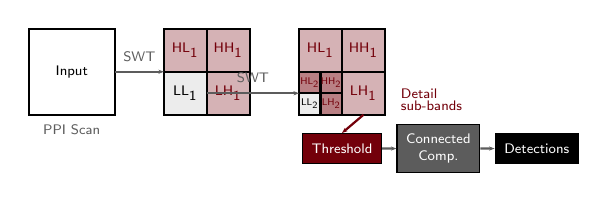
\begin{tikzpicture}[scale=0.78, every node/.style={font=\sffamily\tiny},
  arr/.style={-{Stealth[length=2pt]}, thick, USC_Black70},
  block/.style={draw, fill=#1, text=white, minimum height=0.38cm,
    minimum width=1.0cm, font=\sffamily\tiny, align=center},
  block/.default={USC_Black70}
]
  % Input image
  \draw[thick] (0,0) rectangle (1.4,1.4);
  \node at (0.7,0.7) {Input};
  \node[below, USC_Black70] at (0.7,0) {PPI Scan};

  % Level 1 decomposition
  \coordinate (l1) at (2.2,0);
  % LL1
  \draw[thick, fill=USC_Black10] (l1) rectangle ++(0.7,0.7);
  \node at ($(l1)+(0.35,0.35)$) {LL\textsubscript{1}};
  % LH1
  \draw[thick, fill=USC_Garnet!30] ($(l1)+(0.7,0)$) rectangle ++(0.7,0.7);
  \node at ($(l1)+(1.05,0.35)$) {\color{USC_Garnet}LH\textsubscript{1}};
  % HL1
  \draw[thick, fill=USC_Garnet!30] ($(l1)+(0,0.7)$) rectangle ++(0.7,0.7);
  \node at ($(l1)+(0.35,1.05)$) {\color{USC_Garnet}HL\textsubscript{1}};
  % HH1
  \draw[thick, fill=USC_Garnet!30] ($(l1)+(0.7,0.7)$) rectangle ++(0.7,0.7);
  \node at ($(l1)+(1.05,1.05)$) {\color{USC_Garnet}HH\textsubscript{1}};

  % Arrow input -> level 1
  \draw[arr] (1.4,0.7) -- (2.2,0.7) node[midway, above] {SWT};

  % Level 2 decomposition (of LL1)
  \coordinate (l2) at (4.4,0);
  % LL2
  \draw[thick, fill=USC_Black10] (l2) rectangle ++(0.35,0.35);
  \node[font=\sffamily\tiny] at ($(l2)+(0.175,0.175)$) {\scalebox{0.7}{LL\textsubscript{2}}};
  % LH2
  \draw[thick, fill=USC_Garnet!50] ($(l2)+(0.35,0)$) rectangle ++(0.35,0.35);
  \node[font=\sffamily\tiny] at ($(l2)+(0.525,0.175)$) {\scalebox{0.7}{\color{USC_Garnet}LH\textsubscript{2}}};
  % HL2
  \draw[thick, fill=USC_Garnet!50] ($(l2)+(0,0.35)$) rectangle ++(0.35,0.35);
  \node[font=\sffamily\tiny] at ($(l2)+(0.175,0.525)$) {\scalebox{0.7}{\color{USC_Garnet}HL\textsubscript{2}}};
  % HH2
  \draw[thick, fill=USC_Garnet!50] ($(l2)+(0.35,0.35)$) rectangle ++(0.35,0.35);
  \node[font=\sffamily\tiny] at ($(l2)+(0.525,0.525)$) {\scalebox{0.7}{\color{USC_Garnet}HH\textsubscript{2}}};
  % Remaining L1 detail sub-bands (right and top of L2)
  \draw[thick, fill=USC_Garnet!30] ($(l2)+(0.7,0)$) rectangle ++(0.7,0.7);
  \node at ($(l2)+(1.05,0.35)$) {\color{USC_Garnet}LH\textsubscript{1}};
  \draw[thick, fill=USC_Garnet!30] ($(l2)+(0,0.7)$) rectangle ++(0.7,0.7);
  \node at ($(l2)+(0.35,1.05)$) {\color{USC_Garnet}HL\textsubscript{1}};
  \draw[thick, fill=USC_Garnet!30] ($(l2)+(0.7,0.7)$) rectangle ++(0.7,0.7);
  \node at ($(l2)+(1.05,1.05)$) {\color{USC_Garnet}HH\textsubscript{1}};

  % Arrow LL1 -> level 2
  \draw[arr] ($(l1)+(0.7,0.35)$) -- ($(l2)+(0,0.35)$) node[midway, above] {SWT};

  % Detection pipeline below
  \node[block=USC_Garnet] (thr) at (5.1,-0.55) {Threshold};
  \node[block=USC_Black70, right=0.18cm of thr] (cc) {Connected\\Comp.};
  \node[block=black, right=0.18cm of cc] (det) {Detections};

  % Arrow from detail sub-bands down to threshold
  \draw[arr, USC_Garnet] ($(l2)+(1.05,0)$) -- (thr.north);
  \draw[arr] (thr) -- (cc);
  \draw[arr] (cc) -- (det);

  % Label for detail bands
  \node[USC_Garnet, font=\sffamily\tiny, anchor=west] at ($(l2)+(1.5,0.35)$) {Detail};
  \node[USC_Garnet, font=\sffamily\tiny, anchor=west] at ($(l2)+(1.5,0.15)$) {sub-bands};
\end{tikzpicture}
\end{document}
